\def \eng #1{\foreignlanguage{english}{#1}}

\textbf{Цель работы.}
%
\begin{enumerate}
	\item Изучение принципа действия ЦАП и АЦП и их основных характеристик.
    \item Освоение методов программирования ЦАП и АЦП.
    \item Практическое изучение теоремы о дискретизации на основе задачи цифрового ввода вывода аналоговых сигналов с помощью интерфейсной платы и их последующей цифровой обработки.
\end{enumerate}

\textbf{Аппаратура.} Лабораторный макет генератора сигналов АОН и усилитель низкой частоты, источник питания, 2-х канальный осциллограф, генератор сигналов, интерфейсная плата ЦАП/АЦП, персональный компьютер.

\textbf{Содержание работы.} Эмуляция работы устройства АОН с использованием макета генератора сигналов АОН. Оцифровка и воспроизведение аналоговых сигналов с помощью АЦП и ЦАП, расположенных на интерфейсной плате.

\section{Минимальные теоретические сведения}

\subsection{Аналогово-цифровой и цифро-аналоговый преобразователи}

Процедуры, связанные с преобразованием аналогового сигнала в цифровую форму (дискретизация и квантование), выполняются специальными устройствами --- аналогово-цифровыми преобразователями (АЦП, АЭС). Основными параметрами АЦП являются частота дискретизации и разрядность. Обратная операция, т.е. восстановление аналогового сигнала из последовательности цифровых данных, производится цифро-аналоговым преобразователем (ЦАП, ВАС).

Аналого-цифровые и цифро-аналоговые преобразователи являются неотъемлемой частью систем цифровой обработки сигналов. В настоящее время АЦП и ЦАП представляют собой законченные функциональные устройства в виде интегральных микросхем, в редких случаях требующие установки дополнительных схемных элементов (усилителей, устройств выборки-хранения, интеграторов).

Принцип работы АЦП состоит в измерении уровня входного сигнала в заданный момент времени, его квантовании в соответствии с разрядностью и выдаче результата в цифровой форме. Алгоритм работы АЦП требует некоторого времени на выполнение преобразования и для правильной работы АЦП входной сигнал не должен изменяться в течение времени преобразования, для чего на его входе обычно помещается схема выборки-хранения (УВХ), фиксирующая мгновенный уровень сигнала и сохраняющая его в течение всего времени преобразования. Чтобы исключить перекрытие спектров (при наличии спектральных компонент преобразуемого сигнала или шума, превышающих половину частоты дискретизации $F_d / 2$), и их интерференцию, на входе АЦП требуется установка аналогового фильтра низкой частоты с высокой крутизной среза (антиалиасинговый фильтр).

ЦАП получает на входе цифровое значение и выдает на выходе напряжение (или ток) нужной величины, которое остается постоянным до момента следующего изменения входной цифровой информации. Расположенный за ЦАП интегратор (аналоговый фильтр НЧ) превращает напряжение ступенчатой формы в непрерывный аналоговый сигнал.

В настоящее время известно достаточно большое число методов преобразования аналогового напряжения в цифровой код и обратно. Эти методы существенно отличаются друг от друга потенциальной точностью, скоростью преобразования и сложностью аппаратной реализации.

По типу используемого метода преобразования аналого-цифровые преобразователи обычно разделяют на 3 основных группы: параллельные, последовательные и параллельно-последовательные. По способу построения электронных схем АЦП можно выделить следующие типы:
%
\begin{enumerate}
\item АЦП прямого (параллельного) преобразования;
\item АЦП последовательного счета;
\item АЦП поразрядного уравновешивания (последовательных приближений);
\item интегрирующие АЦП;
\item конвейерные АЦП;
\item сигма-дельта АЦП
\end{enumerate}

Цифро-аналоговые преобразователи также делятся на несколько основных типов:
\begin{enumerate}
\item широтно-импульсный модулятор (простейший тип ЦАП);
\item ЦАП взвешивающего типа;
\item ЦАП лестничного типа (цепная К-2К схема);
\item сегментный ЦАП;
\item ЦАП передискретизации (дельта-сигма ЦАП).
\end{enumerate}

\subsection{Программирование интерфейса АЦП и ЦАП}

Аналого-цифровые и цифро-аналоговые преобразователи подключаются к ЭВМ и микропроцессорным устройствам через специализированные цифровые интерфейсы. Когда необходим ввод/вывод массивов данных, соответствующие интерфейсы обеспечивают хранение или запись данных в буферную память, программирование тактового генератора для обеспечения требуемой частоты дискретизации и некоторые другие сервисные функции.

В случае ввода/вывода единичных отсчетов данных программирование ЦАП заключается в записи цифрового слова в регистр данных ЦАП (данная операция выполняется параллельной или последовательной записью в зависимости от типа буферного регистра данных). Обычно ЦАП не содержат функциональных выводов (сигналов), подтверждающих о готовности принять следующие данные, поэтому следующая запись данных технически возможна сразу после предыдущей записи. Однако любой ЦАП обладает конечным временем установления выходного аналогового сигнала (конечным быстродействием), что необходимо учитывать при программировании.

Программное управление АЦП несколько сложнее, чем ЦАП. Для оцифровки одного отсчета сигнала необходимо сформировать сигнал запуска преобразования (обычно путем записи в соответствующий регистр интерфейса). Затем необходимо дождаться окончания процесса преобразования, программно контролируя значение бита готовности АЦП (обычно при завершении преобразования бит готовности устанавливается в лог. 0). После этого возможно считывание цифровых данных из соответствующего регистра интерфейса. При оцифровке знакопеременных сигналов следует иметь в виду, что шкала преобразования различных АЦП и расположение знакового разряда в цифровом слове могут быть различными, и часто требуется преобразование полученных данных к формату, принятому при представлении целых чисел в ЭВМ.

\subsection{Описание лабораторного макета}

Лабораторный \enquote{Генератор сигналов АОН} (\autoref{fig:maket}, \autoref{fig:maket_scheme}) представляет собой электронную схему, в задачи которой входит анализ состояния линии запроса номера (вход с ЦАП) и формирование ответа (выход на АЦП) в виде тонального сигнала, кодирующего \enquote{номер абонента}.

\begin{figure}[h]%
    \centering
    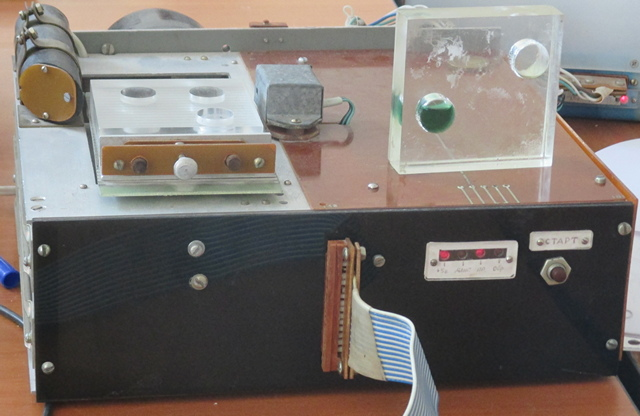
\includegraphics[width=0.8\textwidth]{maket}%
    \caption[]{Внешний вид лабораторного макета}%
    \label{fig:maket}%
\end{figure}
%
\begin{figure}[h]%
    \centering
    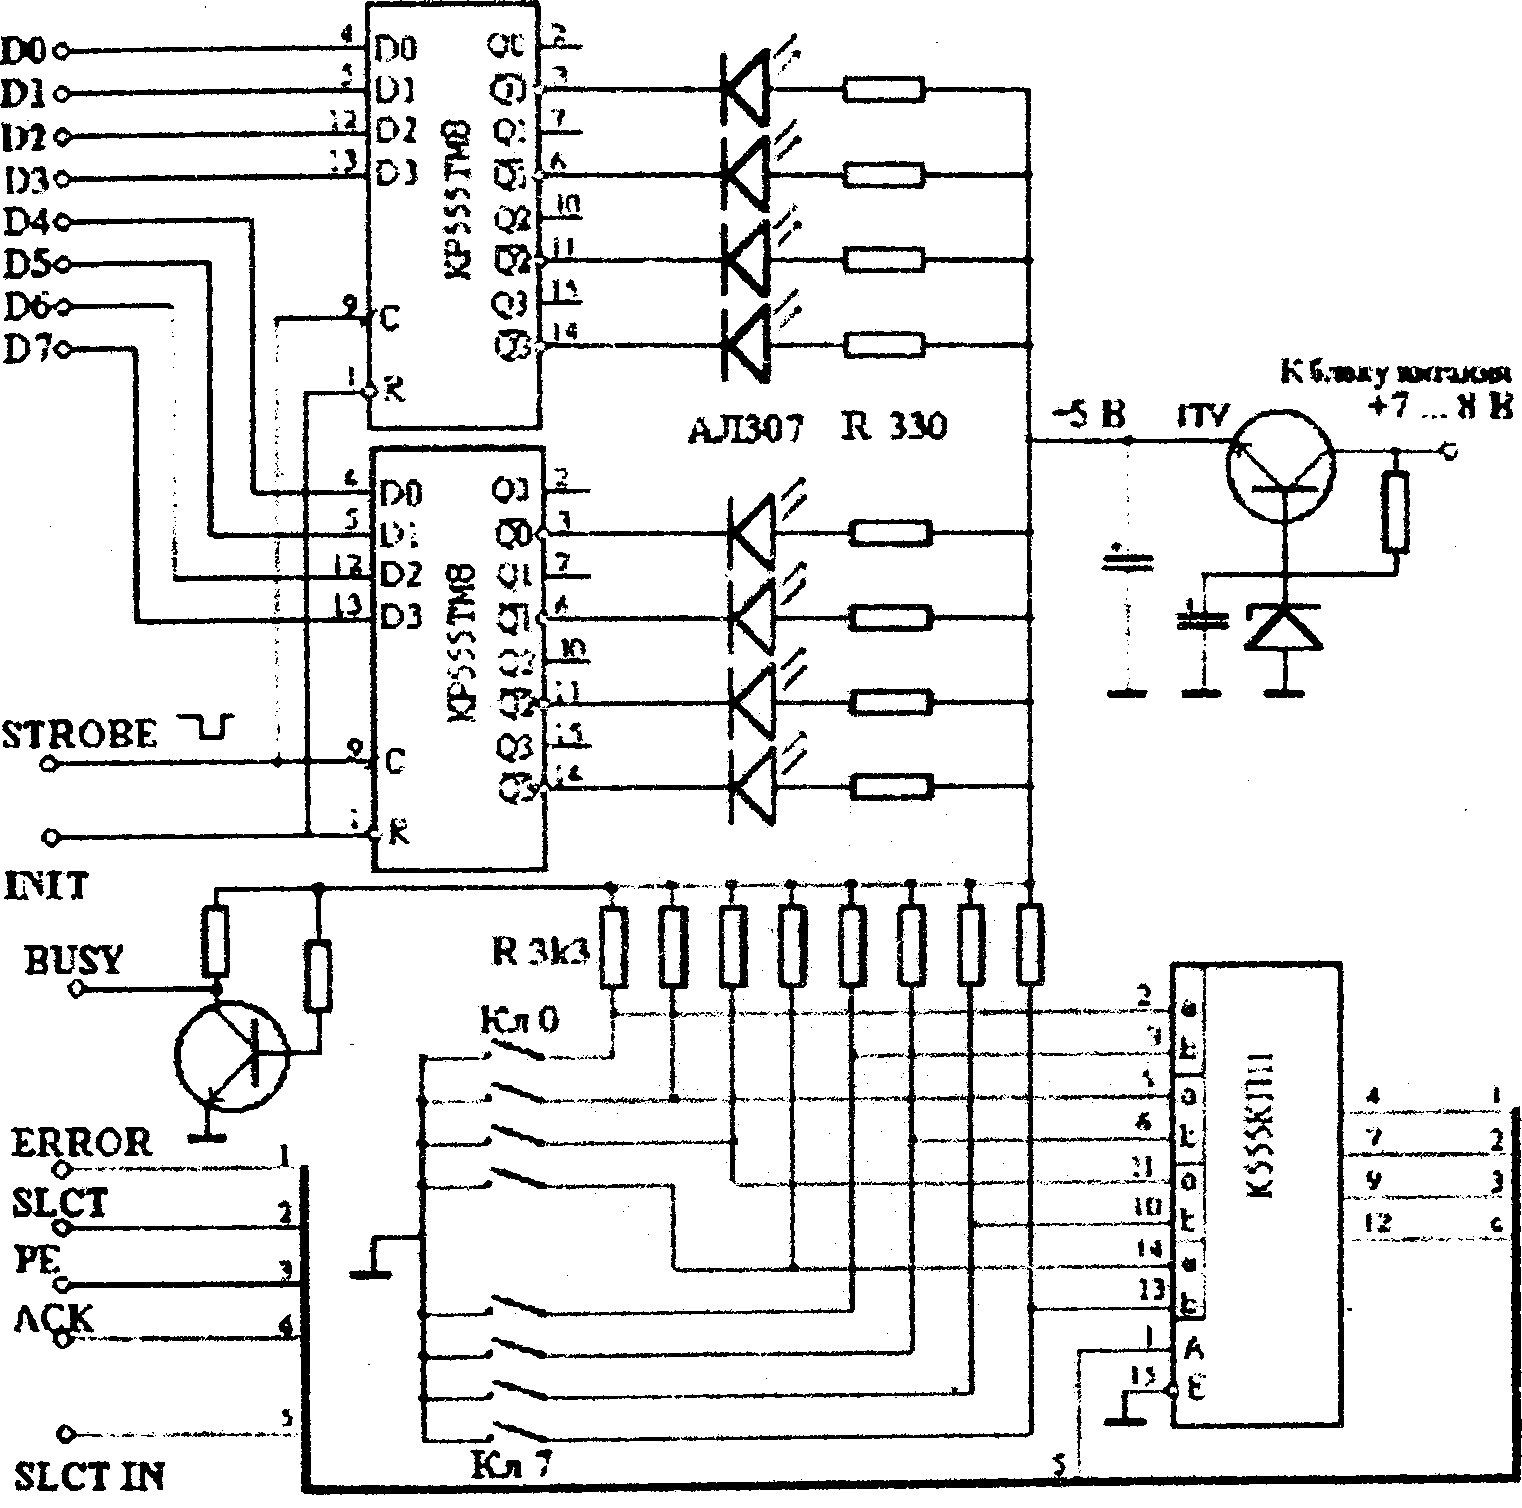
\includegraphics[width=0.8\textwidth]{maket_scheme}%
    \caption[]{Схема лабораторного макета}%
    \label{fig:maket_scheme}%
\end{figure}

Запрос номера должен представлять собой периодический (желательно гармонический) сигнал со следующими параметрами:
%
\begin{enumerate}
\item частота --- $2100 \pm 100 \text{Гц}$;
\item амплитуда --- $3.5 \pm 0.5 \text{В}$;
\item длительность --- $250 \pm 50 \text{мс}$.
\end{enumerate}

Сигнал запроса номера поступает на полосовой фильтр, затем на амплитудный детектор, интегратор и компаратор. При превышении заданного порога компаратор вырабатывает сигнал запуска для формирователя кода номера. В \enquote{генераторе сигналов АОН} также предусмотрена возможность ручного запуска (от кнопки).

Код номера управляет работой делителя частоты и одновременно поступает на индикатор для визуализации текущего числа в формируемом номере. Тональный генератор вырабатывает гармонический сигнал на одной из частот из следующего набора — $[460\text{Гц}, 540\text{Гц}, 650\text{Гц}, 800\text{Гц}]$. Точность задания частоты $\pm 5\%$.

Номер представляет собой четырехзначное число, каждый разряд которого может содержать цифры $[0, 1, 2, 3, 4, 5, 6, 7]$. Номер кодируется однотональным сдвоенным сигналом длительностью $250 + 250 \text{мс} (\pm 20 \text{мс})$, пауза между посылками отдельных разрядов номера $500 \pm 40 \text{мс}$. Четырехзначный номер генерируется датчиком псевдослучайных чисел.

\subsection{Технические характеристики интерфейсной платы ЦАП/АЦП}

Модули ЦАП/АЦП конструктивно размещены на одной интерфейсной 16-разрядной плате в слоте ISA IBM PC.

Разрядность ЦАП --- 10 (используется цифровой код в виде положительных целых чисел).

Диапазон выходных напряжений ЦАП --- $0..4$ В.

Входной сигнал АЦП --- двуполярный, амплитудой до $1$ В.

Разрядность АЦП --- 10 (используется цифровой код в виде положительных целых чисел, середина цифровой шкалы соответствует \enquote{0} входного сигнала).

Интерфейсная плата использует четыре порта в адресном пространстве компьютера. Базовый адрес настраивается переключателями (перемычками) на плате.

\section{Результаты и их обсуждение}

\subsection{Интерфейс программы управления}

Для организации управления и работы с устройством была разработана программа с графическим интерфейсом (\autoref{fig:app}).

\begin{figure}[h]%
\centering
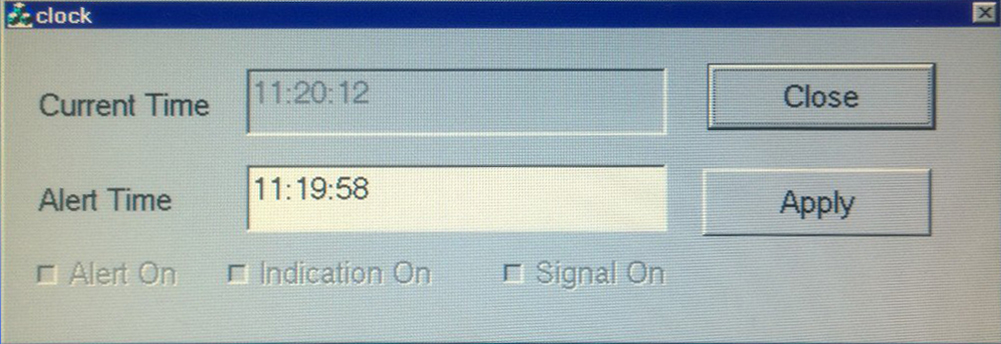
\includegraphics[width=0.8\textwidth]{app}%
\caption[]{Главное окно программы}%
\label{fig:app}%
\end{figure}

При нажатии на кнопку запуска на \enquote{генератор сигналов АОН} посылается запросный сигнал. После чего, по мере поступления закодированных в ответном сигнале цифр, они декодируются и выводятся на экран. Параллельно в промежутках между кодирующими посылками на динамик макета выводится аудиозапись, озвучивающая распознанную цифру.

\subsection{Архитектура программы управления}

Программа управления была написана в среде \eng{Microsoft Visual Studio 6.0} на языке \eng{\tt c++} с использованием библиотеки классов \eng{MFC} (\eng{Microsoft Foundation Classes}).

Для инкапсуляции низкоуровневого программного интерфейса АЦП/ЦАП и проведения работы по декодированию входных сигналов АЦП в цифры были описаны и реализованы два интерфейса (абстрактных класса):
%
\begin{enumerate}
	\item \eng{\tt CDevice} --- инкапсулирует ввод-вывод цифровых сигналов через программный интерфейс интерфейсной платы. Позволяет выдать через на макет через ЦАП запросный сигнал, а также произвольный сигнал, заданный в виде последовательности временн\'{ы}х отсчетов, считать из АЦП в массив временн\'{ы}х отсчетов порцию данных, содержащую единственную кодирующую цифру посылку.
	\item \eng{\tt CEncoder} --- производит обработку и перекодирование цифровых сигналов, их запись в файл и чтение из файла. Позволяет распознать порцию данных, полученную от АЦП и заданную в виде массива отсчетов, как цифру, реализует сохранение массива отсчетов на диск и чтение записанного файла обратно в массив отсчетов, чтение \eng{\tt WAV}-файла и перекодирование его в массив отсчетов, пригодный для выдачи в ЦАП.
\end{enumerate}

Для выдачи сигнала на ЦАП были использованы знания о разрядности ЦАП, предельно допустимой частоте выходного сигнала и его максимальной амплитуде, сигналах управления ЦАП. Для отсчета временн\'{ы}х промежутков использовались функции \eng{Windows API}, предоставляющие доступ к таймеру высокого разрешения.

Для считывания сигнала из АЦП были также использованы знания о его разрядности, сигналах управления АЦП. Перед началом оцифровки каждого отсчета на АЦП подавалась команда запуска, после чего производилось ожидание готовности результата оцифровки по состоянию флага готовности прибора. Затем производилось считывание данных.

Предварительная обработка принятого сигнала заключалась в оценке положения полезного сигнала (посылки) и отсечения (определения и прекращения записи) пауз между посылками. Отсечение производилось пороговым методом с некоторым выбранным порогом по энергии сигнала в пределах окна некоторой выбранной ширины с условием обеспечения оптимального качества определения границ посылки.

Для декодирования принятой посылки в цифру были использованы знания о структуре кодирующего цифру сигнала, а именно что он состоит из двух участков равной длительности, каждый из которых представляет из себя моногармонический сигнал. Дискретное Фурье-преобразование данного сигнала дает два пика, которые соответствуют частотам, содержащимся в посылке. Полученные частоты сопоставляются с таблицей кодов цифр, откуда и определяется соответствующая посылке цифра.

При взятии Фурье-преобразования были приняты в расчет теорема о дискретизации, номиналы допустимых частот в посылке и измеренная производительность (частота дискретизации) АЦП. Исходя из чего были рассчитаны необходимые частота дискретизации и количество отсчетов сигнала для взятия Фурье-преобразования.

\section{Выводы}

В ходе работы была реализована программа, эмулирующая работу АОН.

Были изучены принципы действия ЦАП и АЦП и их основные характеристики, освоены некоторые методы программирования ЦАП и АЦП, практически изучена теорема о дискретизации на основе задачи цифрового ввода вывода аналоговых сигналов с помощью интерфейсной платы и их последующей цифровой обработки.